\documentclass[a4paper]{article}

\renewcommand{\familydefault}{\sfdefault}
\usepackage{xcolor}
\usepackage{tcolorbox} 
\usepackage{sectsty}
\usepackage{graphicx}
\usepackage{enumitem} 
\usepackage{calc}
\usepackage{circuitikz}
\usepackage[ngerman]{babel}
\usepackage{latexsym,amssymb,amsmath}
\usepackage{pdfpages}
\usepackage{siunitx}

\sectionfont{\fontsize{12}{15}\selectfont}

\definecolor{myred}{HTML}{f03e3e}
\definecolor{myblue}{HTML}{1c7ed6}

\newcommand{\complex}[1]{\underline{#1}}

\newcommand{\mumlaut}[1]{\text{\textit{\"#1}}}
\newcommand{\uev}[1]{\textcolor{myred}{\mumlaut{#1}}}

\begin{document}

\begin{center}
  \Large Das einphasige Ersatzschaltbild des Drehstromtransformators
\end{center}

\begin{flushright}
  R.G., 2020
\end{flushright}

\section{Problem}

Physikalisch gesehen sind beide Seiten des Drehstromtransformators (Ober- und Untersseite) über einen \emph{Eisenkern} miteinander gekoppelt. Für praktische Berechnungen eignet sich jedoche eine \emph{galvanische Kopplung} deutlich besser.

\section{Lösung}
Man erhält das Modell des galvanisch gekoppelten DS-Transformators über eine mathematische Umformung der beiden Maschengleichungen und folglicher Rekonstruktion des Schaltbildes aus den umgeformten Gleichungen.

\begin{center}
\begin{circuitikz}[european]


  \draw (0,0) node [transformer](T){}
        (T.A1) node[above] {}
        (T.A2) node[below] {}
        (T.B1) node[above] {}
        (T.B2) node[below] {}
        (T.base) node{M};

  \node (inputA) at (-4,0) {};
  \node (inputB) at (T.A2) {};
  \node (outputA) at (4,0) {};


  \draw (T.B1) --++(1,0) to[R, l=$R_{2}$, i>_=$\complex{I_{2}}$] (outputA);
  \draw (T.B2) to[short] (T.B2) --++ (3,0);
  \draw (T.A1) --++(-1,0) to[R, l=$R_{1}$, i<_=$\complex{I_{1}}$](-4,0);

  \draw (T.A2) to [short] (T.A2) --++ (-3, 0);

  \draw (-4,0) to [open, v>=$\complex{U_{1}}$] (-4, -2.1);
  \draw (outputA) to [open, v^>=$\complex{U_{2}}$] (4, -2.1);

  \draw ($(T.base)+(1mm,-2mm)$)  -- ++(0,-1.8);
  \draw ($(T.base)+(-1mm,-2mm)$) -- ++(0,-1.8);
\end{circuitikz}
\end{center}

\begin{description}[leftmargin=!, labelwidth=\widthof{\bfseries Schritt 1:}]
    \item [Schritt 1:] Aufstellen der beiden Maschengleichungen

    \begin{align}
      \complex{U_1} = \complex{I_{1}} \cdot R_{1} + j \omega L_{1} \cdot \complex{I_{1}} + j \omega M \cdot \complex{I_{2}}\\
      \complex{U_2} = \complex{I_{2}} \cdot R_{2} + j \omega L_{2} \cdot \complex{I_{2}} + j \omega M \cdot \complex{I_{1}}
    \end{align}

  \item [Schritt 2:] Erweiterung der Maschengleichung der Sekundärseite um das Übersetzungsverhältnis

    \begin{align}
      \complex{U_1} &= \complex{I_{1}} \cdot R_{1} + j \omega L_{1} \cdot \complex{I_{1}} + j \omega M \cdot \complex{I_{2}}\\
      \uev{ü} \cdot \complex{U_2} &= \uev{ü}^2 \cdot \frac{\complex{I_{2}}}{\uev{ü}} \cdot R_{2} + j \uev{ü}^2 \cdot \omega L_{2} \cdot \frac{\complex{I_{2}}}{\uev{ü}} + j \omega \uev{ü}^2 \cdot M \cdot \frac{\complex{I_{1}}}{\uev{ü}}
    \end{align}

  \item [Schritt 3:] Anpassung des Terms mit der Gegeninduktivität in der ersten Gleichung an den der zweiten
    \begin{align}
      \complex{U_1} &= \complex{I_{1}} \cdot R_{1} + j \omega L_{1} \cdot \complex{I_{1}} + j \omega \textcolor{myblue}{\text{\textit{ü}}}\cdot M \cdot \frac{\complex{I_{2}}}{\textcolor{myblue}{\text{\textit{ü}}}}\\
      \uev{ü} \cdot \complex{U_2} &= \uev{ü}^2 \cdot \frac{\complex{I_{2}}}{\uev{ü}} \cdot R_{2} + j \uev{ü}^2 \cdot \omega L_{2} \cdot \frac{\complex{I_{2}}}{\uev{ü}} + j \omega \uev{ü}^2 \cdot M \cdot \frac{\complex{I_{1}}}{\uev{ü}}
    \end{align}

    \item[Schritt 4:] Einführung von Kurzschreibweisen (Strichgrößen)
    \[\uev{ü}^2 \cdot R = R', \,\ \uev{ü}^2 \cdot L = L', \,\ \uev{ü} \cdot M = M', \frac{\complex{I}}{\uev{ü}} = \complex{I}', \uev{ü} \cdot \complex{U} = \complex{U}'\]

    \begin{align}
      \complex{U_1} &=
                      \complex{I_{1}} \cdot R_{1}
                      + j \omega L_{1} \cdot \complex{I_{1}}
                      + j \omega M' \cdot \complex{I_{2}}'\\
      \complex{U_2}' &=
                                    \complex{I_{2}}' \cdot R_{2}'
                                    + j \cdot \omega L_{2}' \cdot \complex{I_{2}}'                                    + j \omega M \cdot \complex{I_{1}}
    \end{align}


    \item[Schritt 5:] Einführung ergänzender Größen, um identische Ausdrücke in beiden Gleichungen zu erhalten
    \begin{align}
      \complex{U_1} &=
                      \complex{I_{1}} \cdot R_{1}
                      + j \omega L_{1} \cdot \complex{I_{1}} \textcolor{myred}{-j \omega M' \complex{I_{1}}}
                      + j \omega M' \cdot \complex{I_{2}}' \textcolor{myred}{+ j \omega M' \complex{I_{1}}}\\
      \complex{U_2}' &=
                                    \complex{I_{2}}' \cdot R_{2}'
                       + j \cdot \omega L_{2}' \cdot \complex{I_{2}}' \textcolor{myred}{-j \omega M' \complex{I_{2}}'}
                       + j \omega M \cdot \complex{I_{1}} \textcolor{myred}{+ j \omega M' \complex{I_{2}}'}
    \end{align}

    \item[Schritt 6:] Zusammenfassen der Ausdrücke
    \begin{align}
      \complex{U_{1}} &= R_{1} \cdot \complex{I_{1}}
                        + j \omega (L_{1} - M') \cdot \complex{I_{1}}
                        + j \omega M' (\complex{I_{1}} + \complex{I_{2}'})\\
      \complex{U_{2}}' &= R_{2}' \cdot \complex{I_{2}}'
                         + j \omega (L_{2}' - M') \cdot \complex{I_{2}}'
                         + j \omega M' (\complex{I_{1}} + \complex{I_{2}'})
    \end{align}

    \item[Schritt 5:] Konstruktion des Ersatzschaltbildes aus den beiden neuen Maschengleichungen (11) und (12)

    \begin{center}
      \begin{circuitikz}[european, scale = 0.8]
        \node (inputA) at (0,0) {};
        \node (inputB) at (0,-3) {};

        \node (outputA) at (12, 0) {};
        \node (outputB) at (12, -3) {};

        \draw (inputA) to[R, l=$R_{1}$, i=$\complex{I_{1}}$, o-] (3,0);
        \draw (3,0) to [L, l=$L_{1} - M'$] (6,0);
        \draw (6,0) to [L, l=$M'$, *-*] (6,-3);
        \draw (6,0) to [L, l=$L_{2}' - M'$] (9,0);
        \draw (9,0) to [R, l=$R_{2}'$, i=$\complex{I_{2}'}$, -o] (outputA);

        \draw (inputB) to[short, o-o] (outputB);

        \draw (inputA)  to[open, v=$\complex{U_{1}}$] (inputB);
        \draw (outputA) to[open, v^=$\complex{U_{2}}'$] (outputB);

        \draw (3,-1.5) node[scale=4, color=lightgray]{$\circlearrowright$};
        \draw (3,-1.5) node[color=lightgray]{$(11)$};

        \draw (9,-1.5) node[scale=4, color=lightgray]{$\circlearrowright$};
        \draw (9,-1.5) node[color=lightgray]{$(12)$};

      \end{circuitikz}
    \end{center}

    Da wir die Sekundärgrößen ($I_{2}, U_{2}, L_{2}, R_{2}$) auf die Primärseite bezogen haben ($I_{2}', U_{2}', L_{2}', R_{2}'$), gehört jetzt auf die Sekundärseite noch ein \emph{idealer Übertrager} mit \emph{ü}, der uns dann die realen Sekundärgrößen liefert:

    \begin{center}
      \begin{circuitikz}[european]
        \draw (0,0) node [transformer](T){}
            (T.A1) node[above] {}
            (T.A2) node[below] {}
            (T.B1) node[above] {}
            (T.B2) node[below] {}
            (T.base) node{ü};

        \draw (T.B1) to[open, v^=$\complex{U_{2}}$] (T.B2);

      \end{circuitikz}
    \end{center}

\end{description}

    Das galvanische Ersatzschaltbild, das ja ein fiktives Modell ist, verhält sich nach außen hin (Eingangs- zu Ausgangsgrößen) genauso wie das induktive Ersatzschaltbild, also der reale Transformator.



\includepdf[pages={3}]{mundt.pdf}

\section{Übungen}
\begin{enumerate}

  \item Berechnung der Größen des galvanisch gekoppelten ESBs, Vernachlässigung von $R_{Fe}$
    \[ S_{n} = 400 \, \si{\kilo\volt\ampere}, \mumlaut{ü} = 10 \, \si{\kilo\volt}/0.4\,\si{\kilo\volt}\]
    \[R_{1} = 77 \, \si{\milli\ohm}, R_{2} = 5.1 \, \si{\milli\ohm}\]
    \[L_{1} = 4.52 \, \si{\henry}, L_{2} = 7.25 \, \si{\milli\henry}\]
    \[M = 180 \, \si{\milli\henry}\]

    \begin{enumerate}
        \item Widerstände
        \[R_1 = R_{1} = 77 \, \si{\milli\ohm}\]
        \[R_2' = R_{2} \cdot \mumlaut{ü}^{2} =  5.1 \, \si{\milli\ohm} \cdot 25^2 = 3.188 \, \si{\ohm}\]

        \item Selbstinduktivitäten
        \[L_{1} = L_{1} = 4.52 \, \si{\henry}\]
        \[L_{2}' = L_{2} \cdot \mumlaut{ü}^{2} = 7.25 \, \si{\milli\henry} \cdot 25^2= 4.531 \, \si{\henry}\]

        \item Gegeninduktivität
        \[M' = M \cdot \mumlaut{ü} = 180 \, \si{\milli\henry} \cdot 25 = 4.5 \, \si{\henry}\]


        \item Als Reaktanzen:
        \[X_{1} = j \omega (L_{1} - M') = j 2 \pi 50 \si{\hertz} \cdot (4.52 - 4.5) \, \si{\henry} = j 6.283 \, \si{\ohm}\]
        \[X_{2} = j \omega (L_{2}' - M') = j 2 \pi 50 \si{\hertz} \cdot (4.531 - 4.5) \, \si{\henry} = j 9.739 \, \si{\ohm}\]
        \[X_{n}' = j \omega M' = 1413.717 \, \si{\ohm}\]

        \begin{center}
        \begin{circuitikz}[european, scale = 0.8]
            \node (inputA) at (0,0) {};
            \node (inputB) at (0,-3) {};

            \node (outputA) at (12, 0) {};
            \node (outputB) at (12, -3) {};

            \draw (inputA) to[R, l=$77 \, \si{\milli\ohm}$, i=$\complex{I_{1}}$, o-] (3,0);
            \draw (3,0) to [L, l=$20 \, \si{\milli\henry}$] (6,0);
            \draw (6,0) to [L, l=$4.5 \, \si{\henry}$, *-*] (6,-3);
            \draw (6,0) to [L, l=$31 \, \si{\milli\henry}$] (9,0);
            \draw (9,0) to [R, l=$3.188 \, \si{\ohm}$, i=$\complex{I_{2}'}$, -o] (outputA);

            \draw (inputB) to[short, o-o] (outputB);

            \draw (inputA)  to[open, v=$\complex{U_{1}}$] (inputB);
            \draw (outputA) to[open, v^=$\complex{U_{2}}'$] (outputB);

        \end{circuitikz}
        \end{center}

    \end{enumerate}

    Der ideale Übertrager ist nicht dargestellt.

    \item Symmetrische Belastung des Transformators in jeder Phase

        \begin{enumerate}
            \item Belastung mit $\complex{Z} = 350 \si{\milli\ohm} + j 330 \si{\milli\ohm}$
            \item Spannung über Verbraucher (Sekundärseitig): $0.4 \, \si{\kilo\volt}$ (Nennwert, s.o.)
            \item Ermittlung aller Strom- und Spannungsgrößen und deren Zeigerbild
            \begin{enumerate}
              \item Wir befinden uns im \emph{EINPHASIGEN} ESB. Die Spannung $U_{2}'$ ist die Strangspannung
                \[U_{2}' = \frac{10 \, \si{\kilo\volt}}{\sqrt{3}}\]
              und die Spannung $U_{2}$ ist die Strangspannung
                \[U_{2} = \frac{0.4 \, \si{\kilo\volt}}{\sqrt{3}}\]
            \end{enumerate}
        \end{enumerate}

        \begin{center}
        \begin{circuitikz}[european, scale = 0.8]
            \node (inputA) at (0,0) {};
            \node (inputB) at (0,-3) {};

            \node (outputA) at (12, 0) {};
            \node (outputB) at (12, -3) {};

            \draw (inputA) to[R, l=$77 \, \si{\milli\ohm}$, i=$\complex{I_{1}}$, o-] (3,0);
            \draw (3,0) to [L, l=$20 \, \si{\milli\henry}$] (6,0);
            \draw (6,0) to [L, l=$4.5 \, \si{\henry}$, *-*] (6,-3);
            \draw (6,0) to [L, l=$31 \, \si{\milli\henry}$] (9,0);
            \draw (9,0) to [R, l=$3.188 \, \si{\ohm}$, i=$\complex{I_{2}'}$, -o] (outputA);

            \draw (outputA) to[R, l=$\complex{Z'}$] (outputB);

            \draw (inputB) to[short, o-o] (outputB);

            \draw (inputA)  to[open, v=$\complex{U_{1}}$] (inputB);
            \draw (13,0) to[open, v^=$\complex{U_{2}}'$] (13,-3);

        \end{circuitikz}
        \end{center}

    Belastung mit $\complex{Z}$ an der Sekundärseite des idealen Übertragers (nicht eingezeichnet). Wandlung zu $\complex{Z'}$.\\


    \noindent \underline{Wiederholung}: Impedanzwandlung beim idealen Übertrager
    \begin{enumerate}
        \item Die Leistung auf beiden Seiten des Übertragers ist gleich.
        \[S_{1} = S_{2}\]
        \[\complex{U_{1}} \cdot \complex{I_{1}} =  \complex{U_{2}} \cdot \complex{I_{2}} \]

      \item Es gilt
        \[\mumlaut{ü} = \frac{U_{1}}{U_{2}} = \frac{I_{2}}{I_{1}}\]

      \item sowie
        \[\frac{U_{1}}{I_{1}} = \complex{Z_{1}}, \, \text{Eingangsseitig gesehene Impedanz}\]
        \[\frac{U_{2}}{I_{2}} = \complex{Z_{2}}, \, \text{Ausgangsseitig gesehene Impedanz}\]

      \item (a) in (b)
        \[ \frac{{U_{1}}}{U_{2}} = \frac{I_{1} \cdot \mumlaut{ü}}{\dfrac{I_{2}}{\mumlaut{ü}}}\]
        \[ \frac{{U_{1}}}{I_{1}} = \frac{U_{2}}{I_{2}} \cdot \mumlaut{ü}^2\]
        \[Z_{1} = Z_{2} \cdot \mumlaut{ü}^{2}\]
    \end{enumerate}

    Dadurch ist die eingangsseitige Impedanz $Z'$
    \[Z' = {Z}\cdot \mumlaut{ü}^{2} = (350 + j330)\si{\milli\ohm}\cdot 25^2\]

    Da Spannung und Impedanz bekannt sind (Spannung wird einfach zum Winkel $0$ definiert), kann der Strom $I_{2}'$ berechnet werden. Darüber lassen sich dann auch alle weiteren Ströme und Spannungen berechenen. Letztendlich kommt man auf eine Eingangsspannung von
    \[\complex{U_{1}} = 6.058 \, \si{\kilo\volt} \cdot e^{j 1.7 \si{\degree}}\]

    Bei rein ohmscher Belastung ($Z = 350 \, \si{\milli\ohm}$) ist
    \[\complex{U_{1}} = 5.901 \, \si{\kilo\volt} \cdot e^{j 4.12 \si{\degree}}\]

    Bei rein induktiver Belastung ($Z = j330 \, \si{\milli\ohm}$) ist
    \[\complex{U_{1}} = 6.250 \, \si{\kilo\volt} \cdot e^{-j 0.85 \si{\degree}}\]

    Bei ohmsch-kapazitiver Belastung ($Z = (350 - j 330) \, \si{\milli\ohm}$) ist
    \[\complex{U_1} = 5.640 \, \si{\kilo\volt} \cdot e^{j 2.72 \si{\degree}}\]

    \item Aus dem Netz entnommene Scheinleistung und Wirkleistungsverluste im Transformator

    \begin{enumerate}

      \item Die Spannung $U_{1}$ ist die Strangspannung. Die Leiter-Leiter-Spannung beträgt
        \[U_{1_{LL}} = \sqrt{3} \cdot 6.058 \, \si{\kilo\volt} = 10.49 \, \si{\kilo\volt}\]
        
        \item Scheinleistung ($Z = (350 + j 330)\si{\milli\ohm}$):
              \[S_{ges} = 3 \cdot \complex{U_{1}} \cdot \complex{I_{1}}^{*} = \sqrt{3} \cdot \complex{U_{1_{LL}}} \cdot \complex{I_{1}}^{*}\]
        \[S_{ges} = 406 \, \si{\kilo\volt\ampere} \cdot e^{j 52.7 \, \si{\degree}}\]

        \item Wirkleistungsverluste im Transformator ($Z'$ zählt nicht dazu!!)
        \[P_{Vi}   = R_{1} \cdot I_{1}^{2} + R_{2} \cdot I_{2}'^{2} = 1215 \, \si{\watt}\]
        \[P_{Vges} = 3 \cdot P_{Vi} = 3644 \, \si{\watt}\]
        
    
    \end{enumerate}

\end{enumerate}

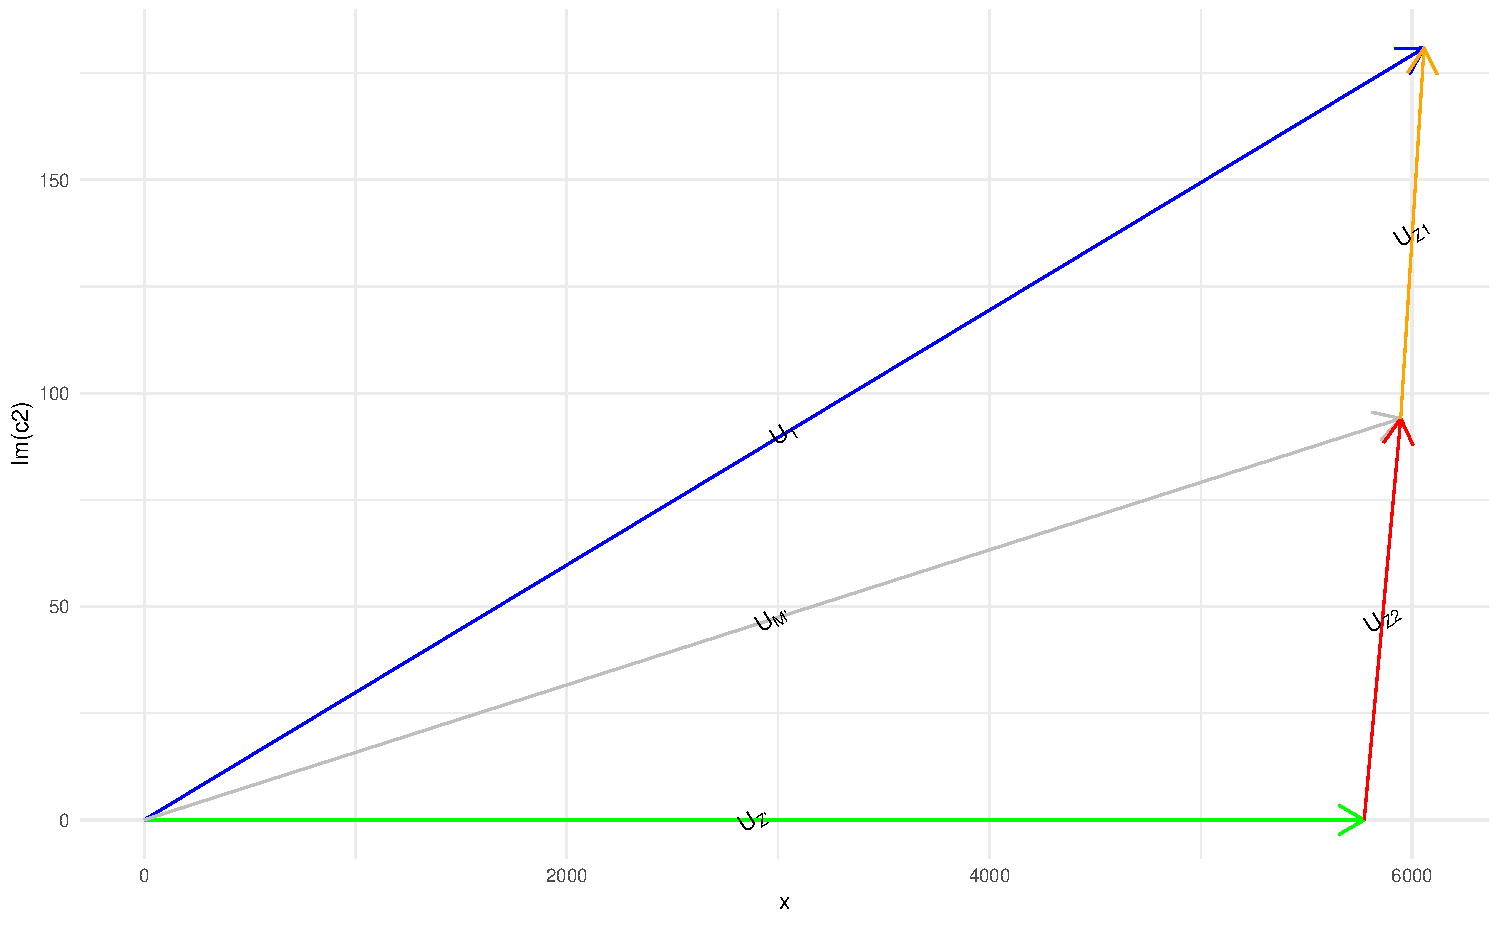
\includegraphics[width=\textwidth]{zeigerbild.pdf}


\end{document}
